\documentclass[journal,12pt,twocolumn]{IEEEtran}

% Packages
\usepackage{cite}
\usepackage{amsmath,amssymb,amsfonts,amsthm}
\usepackage{algorithmic}
\usepackage{graphicx}
\usepackage{textcomp}
\usepackage{xcolor}
\usepackage{txfonts}
\usepackage{listings}
\usepackage{enumitem}
\usepackage{mathtools}
\usepackage{float}
\usepackage{gensymb}
\usepackage{comment}
\usepackage{hyperref}
\usepackage{tkz-euclide}
\usepackage{listings}
\usepackage{gvv}
\usepackage[latin1]{inputenc}
\usepackage{color}
\usepackage{array}
\usepackage{longtable}
\usepackage{calc}
\usepackage{multirow}
\usepackage{hhline}
\usepackage{ifthen}
\usepackage{lscape}
\usepackage{subcaption}
\usepackage{tikz}
\usepackage{circuitikz}

% Custom commands and macros
\newtheorem{theorem}{Theorem}[section]
\newtheorem{problem}{Problem}
\newtheorem{proposition}{Proposition}[section]
\newtheorem{lemma}{Lemma}[section]
\newtheorem{corollary}[theorem]{Corollary}
\newtheorem{example}{Example}[section]
\newtheorem{definition}[problem]{Definition}
\newtheorem{rem}{Remark}
\newcommand{\BEQA}{\begin{eqnarray}}
\newcommand{\EEQA}{\end{eqnarray}}
\newcommand{\define}{\stackrel{\triangle}{=}}
\renewcommand{\thefigure}{\theenumi}
\renewcommand{\thetable}{\theenumi}

% Document
\begin{document}

\title{GATE 2023 EC 49}
\author{EE23BTECH11045 - Palavelli Srija$^{*}$}
\maketitle

\bigskip

\textbf{Question 12.7.7:} 
Let $x(t) = 10 \cos(10.5 \omega t)$ be passed through an LTI system with impulse response $h(t) = \pi\left(\frac{\sin(\omega t)}{\pi t}\right)^2 \cos(10 \omega t)$ . The output of the system is: \\

\textbf{Solution:}
\begin{table}[h!]
    \centering
    \begin{tabular}{|c|c|c|}    \hline
     \textbf{Symbol} & \textbf{Description} &     \textbf{Value}\\
    \hline     $x(t)$ &  input &  $10 \cos(10.5 \omega t)$\\[6pt]
    \hline      $h(t)$ & impulse & $\pi\left(\frac{\sin(\omega t)}{\pi t}\right)^2 \cos(10 \omega t)$ \\[6pt]
    \hline     $y(t)$ &  output & ??\\[6pt]
    \hline     
\end{tabular}

    \caption{Input Parameters}
    \label{tab:table_sr4}
\end{table}

Given \(h(t)\) is Real and Even. 
\[
x(t) \xrightarrow{\text{}} \boxed{\text{h(t)}} \xrightarrow{\text{}} y(t)
\]

\begin{align}
y(t) &= H(\omega)\bigg|_{\omega=10.5\omega} \cdot 10 \cos(10.5 \omega t) \\
h(t) &= f(t) \cos(10 \omega t) \\
f(t) &= \pi\left(\frac{\sin(\omega t)}{\pi t}\right)^2 
\end{align}

The Fourier transform of \(f(t)\):
\begin{align}
f(t) \xleftrightarrow{\mathcal{F}} F(\omega)\\
F(\omega)&= \pi\int_{-\infty}^{\infty}\left(\frac{\sin(\omega t)}{\pi t}\right)^2e^{-j\omega t}\,dt 
\end{align}
\begin{figure}[ht!]
    \centering
    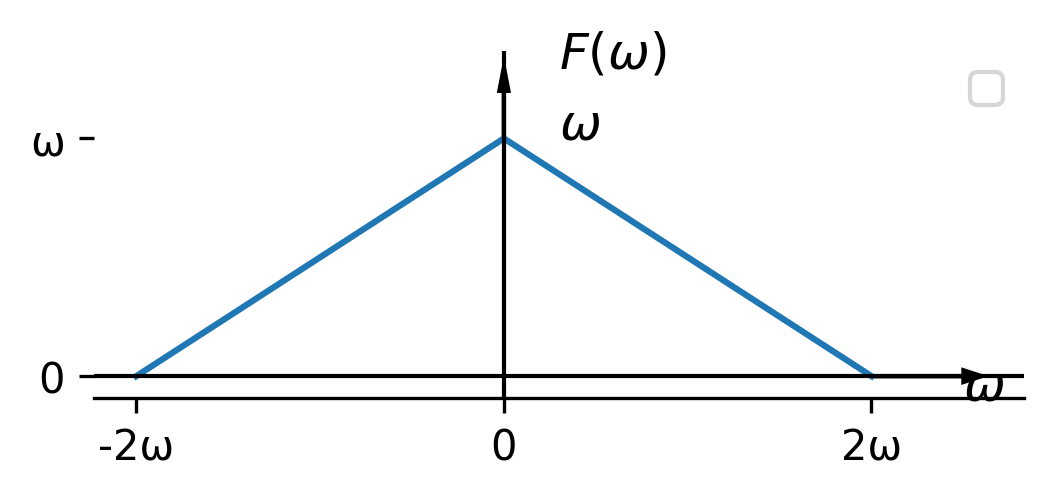
\includegraphics[width=\columnwidth]{figs/plot2.png}
    \caption{}
    \label{fig:sr2}
\end{figure}

\newpage
The frequency response \(H(\omega)\):
\begin{align}
H(\omega) &= \frac{1}{2} \left[F(\omega + 10\omega) + F(\omega - 10\omega)\right] 
\end{align}
\begin{figure}[ht!]
    \centering
    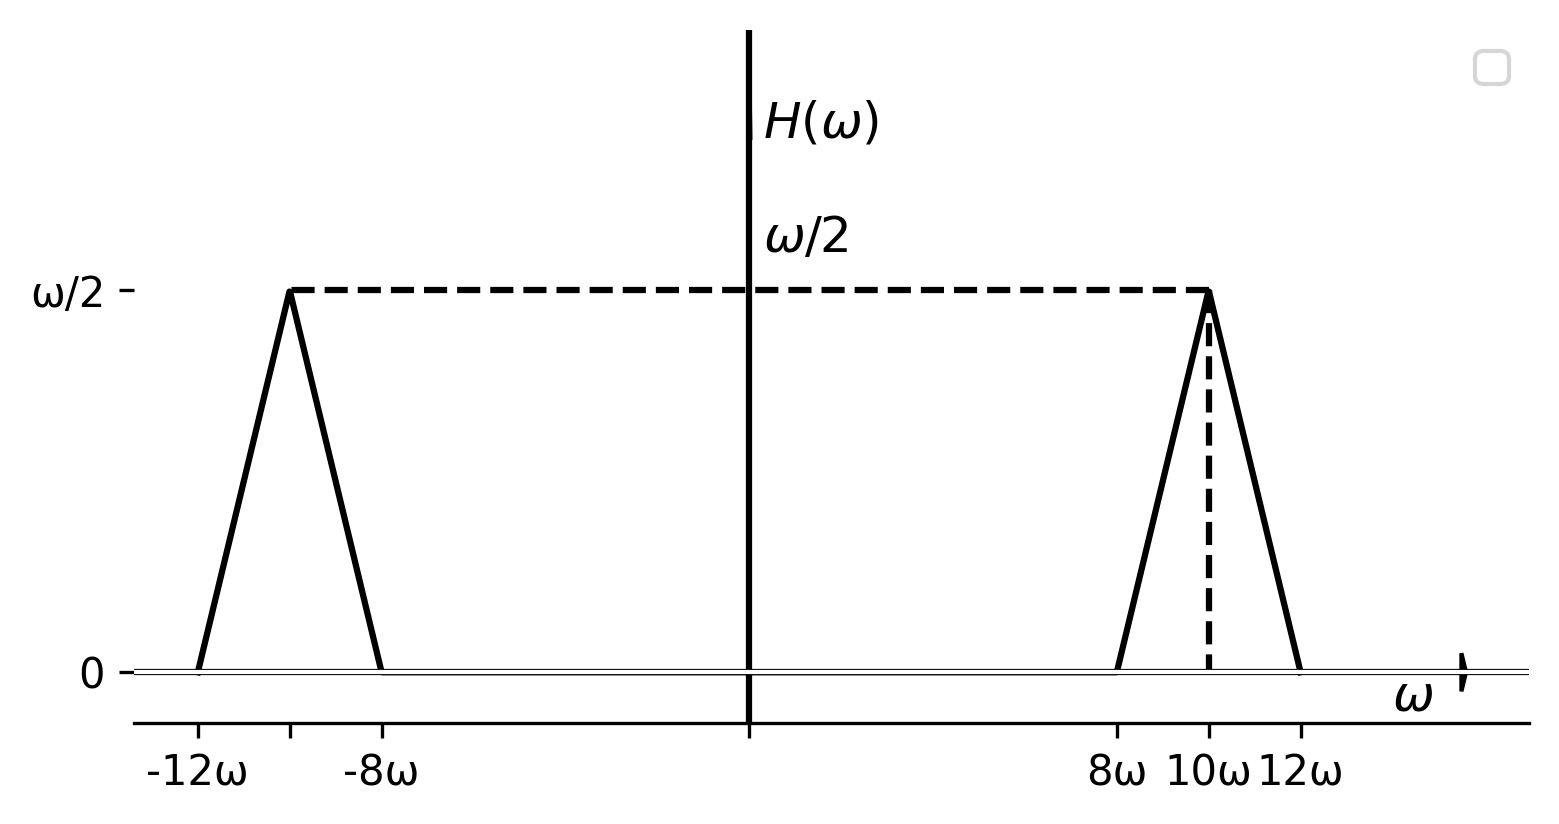
\includegraphics[width=\columnwidth]{figs/plot3.png}
    \caption{}
    \label{fig:sr3}
\end{figure}

\begin{align}
H(\omega)\bigg|_{\omega=10.5\omega} = \frac{3}{8}\omega
\end{align}

The output \(y(t)\):
\begin{align}
y(t) &= \frac{3}{8}\omega \cdot 10 \cos(10.5 \omega t) \\
&= \frac{15}{4}\omega \cos(10.5 \omega t)
\end{align}

\end{document}
